% !TEX options=--shell-escape
\documentclass[12pt]{article}
\usepackage[utf8]{inputenc}
\usepackage{lipsum}
\usepackage{afterpage}
\usepackage{mathtools}
\usepackage{xcolor}
\usepackage[12pt]{extsizes}
\usepackage[english,russian]{babel}
\usepackage{cite}
\usepackage{minted}
\usepackage{amsmath, esint, setspace, fancyhdr, amsfonts, bookmark, blindtext}
\usepackage{graphicx}
\usepackage{subfigure}
\usepackage{titlesec}

\graphicspath{{Figures/}}
\DeclareGraphicsExtensions{.pdf,.png,.jpg}
\usemintedstyle{tango}
\definecolor{dhscodebg}{rgb}{0.95,0.95,0.95}


\setlength{\textheight}{8in}
\setlength{\textwidth}{6.6in}
\setlength{\headheight}{0in}
\setlength{\headsep}{0.2in}
\setlength{\topmargin}{0in}
\setlength{\oddsidemargin}{0in}
\setlength{\evensidemargin}{0in}
\setlength{\parindent}{.3in}

\doublespacing
\renewcommand{\baselinestretch}{1.4} 

\begin{document}
\begin{titlepage}

\begin{center}
Санкт-Петербургский политехнический университет Петра Великого\\
Институт прикладной математики и механики\\
Кафедра прикладной математики\\
\end{center}


\vspace{2.5cm}

\begin{center}
{\large {\bfseries СВОДНЫЙ ОТЧЕТ}}\\

\bigskip \bfseries{Тема:} {\bfseries \emph{Многомерные распределения.\\ Оценки характеристик распределений}}
\end{center}

\vspace{1.5cm}

\begin{flushleft}
Направление: 01.03.02 Прикладная математика и информатика

\vspace{1.5cm}

Выполнил студент гр. 33631/4 \hfill{Камалетдинова Ю.} \\ 

\vspace{0.5cm} Преподаватель \hfill{Баженов А.}
\vspace{1cm}

\end{flushleft}

\vspace{2.7cm}

\begin{center}
Санкт-Петербург\\
2019
\end{center}

\end{titlepage}



\tableofcontents
\addtocontents{toc}{~\hfill\par}
\vfill ~
\setcounter{section}{0}


%%%%%%%%%%%%%%%%%%%%%%%%%%%%%%%%%%%%%%%%%%

\newpage 
\section*{Постановка задачи}
\addcontentsline{toc}{section}{Постановка задачи}
\indent{\indentЗадачей данной работы является рассмотрение такого способа выявления выбросов как боксплот. Требуется сгенерировать выборки размерами $n = 20, 100$ и построить для них боксплот Тьюки. Для каждого распределения нужно определить процент выбросов экспериментально, сгенерировав выборку из распределения $N =1000$ раз и вычислив средний процент выбросов, а затем сравнить с результатами, полученными теоретически. Рассматриваемые законы распределения приведены ниже}

\begin{equation}
	\label{dist:1}
	N(x, 0, 1) = \frac{1}{\sqrt{2\pi}}e^{-\frac{x^2}{2}} \;\text{-- стандартное нормальное}
\end{equation}
 
\begin{equation}
	C(x, 0, 1) = \frac{1}{\pi(1 + x^2)} \;\text{-- Коши} \label{dist:2}
\end{equation}

\begin{equation}
	L(x, 0, \frac{1}{\sqrt{2}}) = \frac{1}{\sqrt{2}}e^{{-\sqrt{2}|x|}} \;\text{-- Лаплас} \label{dist:3}
\end{equation}

\begin{equation} 
	U(x, -\sqrt{3}, \sqrt{3}) = 
    \begin{cases}
        \frac{1}{2\sqrt{3}}, \: |x| \leq \sqrt{3}\\
        \;\; 0, \:\:\:|x| > \sqrt{3}
    \end{cases}
    \;\text{-- равномерное} \label{dist:4}
\end{equation}

\begin{equation}
    P(\lambda) = \frac{e^{-\lambda}}{k!}\lambda^k , \; \lambda = 7\;\text{-- Пуассон} \label{dist:5}
\end{equation}


%%%%%%%%%%%%%%%%%%%%%%%%%%%%%%%%%%%%%%%%%%

\section*{Описание метода}
\addcontentsline{toc}{section}{Описание метода}
\indent{\indent\textit{Выброс} -- это некое наблюдение, которое нехарактерно далеко удалено от других значений в общей случайной выборке. В некотором смысле, это определение оставляет на усмотрение наблюдателя решение вопроса о том, что будет считаться выбросом. } 

\indent{Боксплот является удобным графическим способом описания поведения данных как в середине, так на концах распределения. Боксплот визуализирует положение медианы, нижнего и верхнего квартилей. Первый квартиль $Q_1$ определяется как медиана части выборки до медианного элемента всей выборки, третий квартиль $Q_3$ -- медиана части выборки после медианного элемента всей выборки.} 

\indent{На графике присутствуют усы, границы которых определяются формулами}
\begin{equation}
    \label{q:1} 
    x_L = max(x_{(1)},\; Q_1 - 1.5 \cdot IQR)\text{ -- нижняя граница уса}
\end{equation}

\begin{equation}
    \label{q:2} 
    x_U = min(x_{(n)},\; Q_3 + 1.5 \cdot IQR)\text{ -- верхняя граница уса}
\end{equation}

\begin{equation}
    \label{q:3} 
    IQR = Q_3 - Q_1   \text{ -- интерквартильная широта}
\end{equation}

\indent{Будем считать элемент $x_i$ выбросом, если $x_i \notin [x_L, x_U]$}

\indent{Для сравнения теоретических и практических результатов вычислим квартили для непрерывных распределений. Квартили однозначно определяются уравнением}

\begin{equation}
    \label{q:4}
    F_X(x_{\alpha}) = \alpha \text{,\;\;} \alpha = \left\{ \frac{1}{4}, \; \frac{3}{4} \right\}
\end{equation}

\indent{Искомые квартили можно выразить, найдя обратную функцию к функции распределения.}

\indent{Вычисление доли выбросов будем производить по формуле}
\begin{equation}
\label{q:5}
    p_{outliers} = \frac{\sum_{i}^{} x_i}{\sum_{j = 1}^{n} x_j}, \; i: x_i \notin [x_L, x_U] 
\end{equation}

%%%%%%%%%%%%%%%%%%%%%%%%%%%%%%%%%%%%%%%%%%

\section*{Реализация }
\addcontentsline{toc}{section}{Реализация}
\indent{\indentДля выполнения поставленной задачи будем пользоваться библиотеками для языка Python: \textit{numpy, scipy} -- расчеты, законы распределения вероятностей; \textit{matplotlib, seaborn} -- визуализация результатов. Ход работы:}
\begin{itemize}
    \item Задаем распределение с заданными параметрами 
    \item Генерируем случайные выборки из распределений размерами $n = 20, 100$
    \item Для каждого из распределений вычисляем доли выбросов $N = 1000$ раз
    \item Вычисляем теоретические квартили при помощи метода \textit{.ppf($\alpha$)} (percent point function) - функция, обратная функции распределения, вычисляем доли выбросов с использованием данных квартилей
    \item Усредняем полученные суммы долей выбросов, разделив на $N = 1000$ 
\end{itemize}

%%%%%%%%%%%%%%%%%%%%%%%%%%%%%%%%%%%%%%%%%%

\newpage
\section*{Результат}
\addcontentsline{toc}{section}{Результат}

\textbf{Нормальное распределение} с параметрами 0, 1\\
\begin{center}
    \begin{tabular}{ c | c | c }
        $$ & Практическая доля выбросов & Теоретическая доля выбросов  \\ \hline
        $n = 20$ & 0.0222 & 0.0070 \\ \hline
        $n = 100$ & 0.0099 & 0.0070 \\ 
    \end{tabular}
\end{center}

\begin{figure}[h!]
\centering
\center{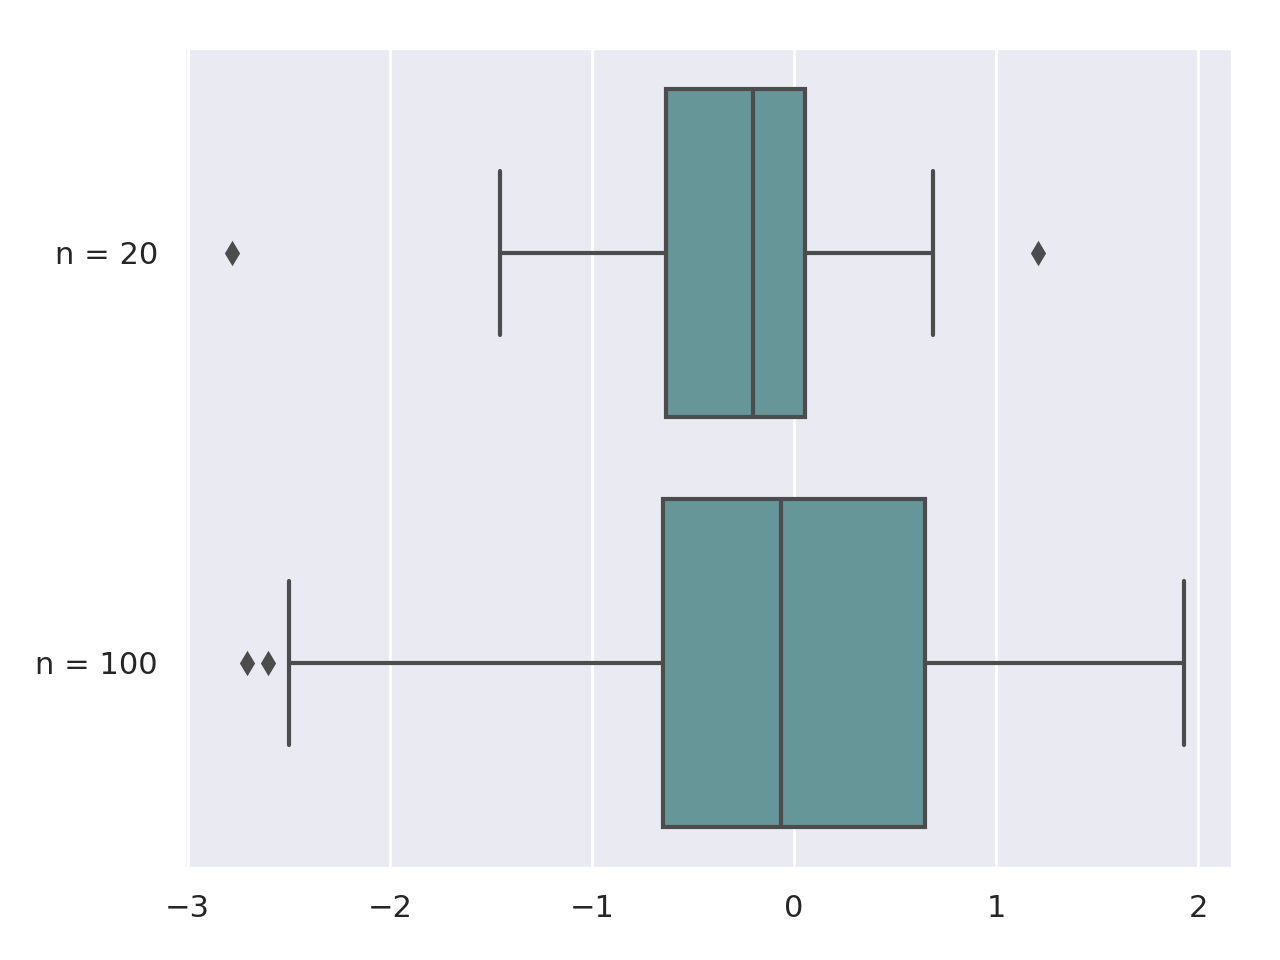
\includegraphics[width=13.cm, height=10.cm]{norm}}
\label{pic:1}
\caption{Боксплот Тьюки для выборок из нормального распределения}
\end{figure}
\vspace{4.cm}

\textbf{Равномерное распределение} на отрезке $[-\sqrt{3}, \sqrt{3}]$
\\
\begin{center}
    \begin{tabular}{ c | c | c }
        $$ & Практическая доля выбросов & Теоретическая доля выбросов  \\ \hline
        $n = 20$ & 0.0027 & 0.0000 \\ \hline
        $n = 100$ & 0.0000 & 0.0000 \\ 
    \end{tabular}
\end{center}

\begin{figure}[h!]
\centering
\center{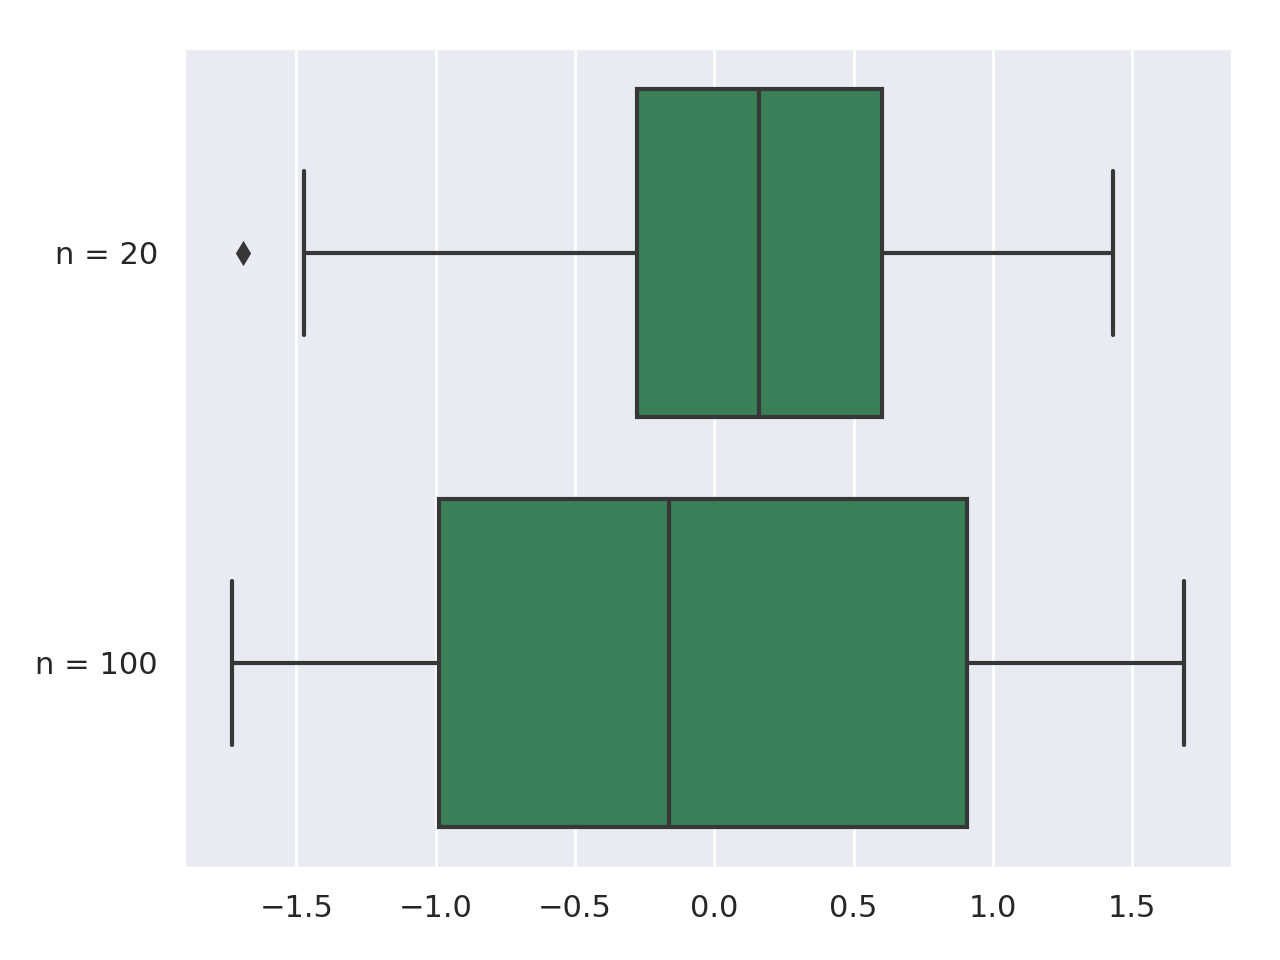
\includegraphics[width=13.cm, height=10.cm]{unif}}
\label{pic:2}
\caption{Боксплот Тьюки для выборок из равномерного распределения}
\end{figure}
\vspace{5.cm}

\textbf{Распределение Коши} с параметрами 0, 1
\\
\begin{center}
    \begin{tabular}{ c | c | c }
        $$ & Практическая доля выбросов & Теоретическая доля выбросов  \\ \hline
        $n = 20$ & 0.1525 & 0.1574 \\ \hline
        $n = 100$ & 0.1558 & 0.1562 \\ 
    \end{tabular}
\end{center}

\begin{figure}[h!]
\centering
\center{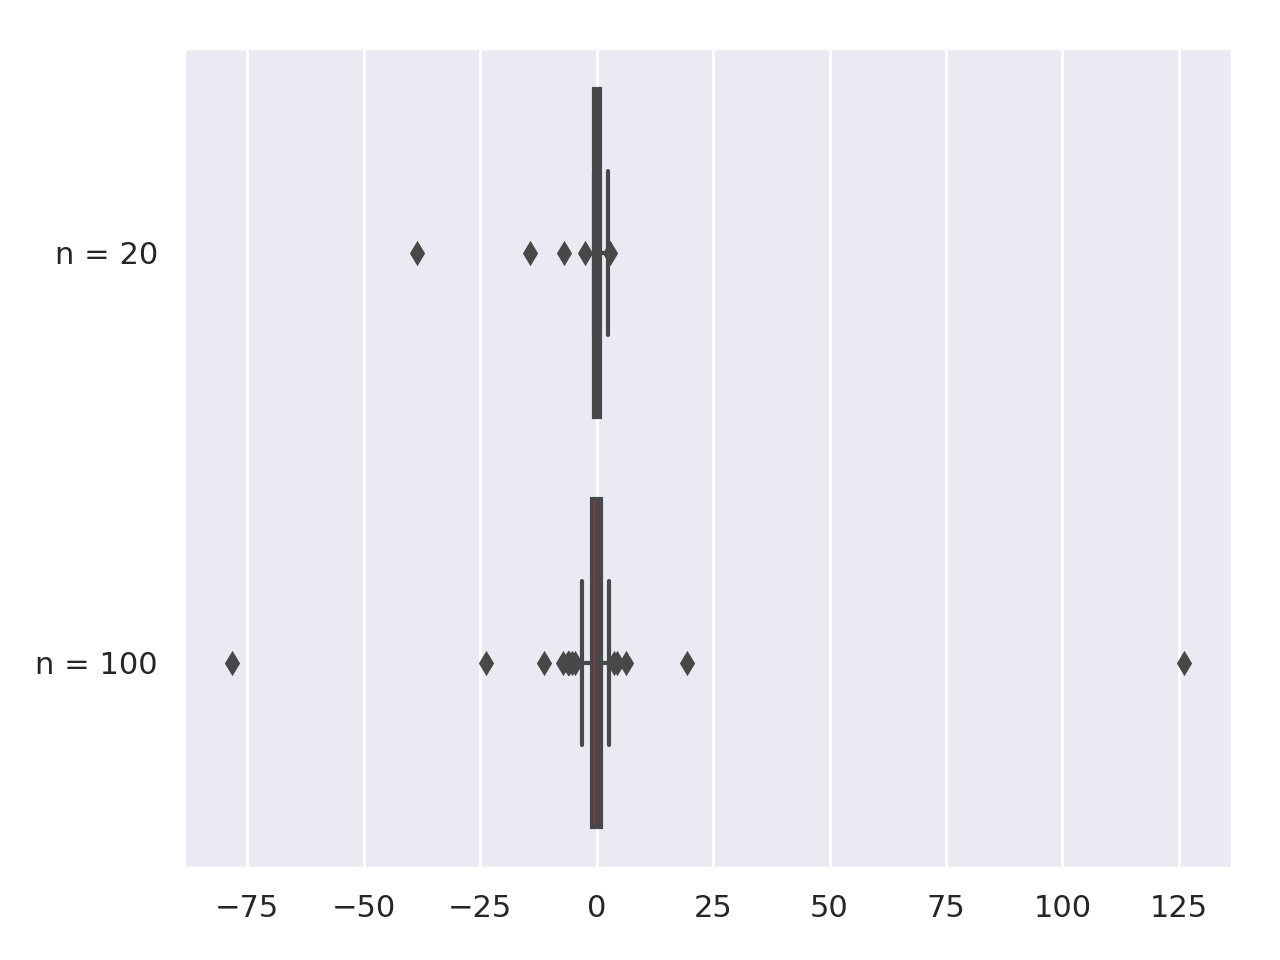
\includegraphics[width=13.cm, height=10.cm]{cauch}}
\label{pic:3}
\caption{Боксплот Тьюки для выборок из распределения Коши}
\end{figure}
\vspace{5.cm}

\textbf{Распределение Лапласа} с параметрами 0, $\frac{1}{\sqrt{2}}$
\\
\begin{center}
    \begin{tabular}{ c | c | c }
        $$ & Практическая доля выбросов & Теоретическая доля выбросов  \\ \hline
        $n = 20$ & 0.0749 & 0.0608 \\ \hline
        $n = 100$ & 0.0642 & 0.0610 \\ 
    \end{tabular}
\end{center}

\begin{figure}[h!]
\centering
\center{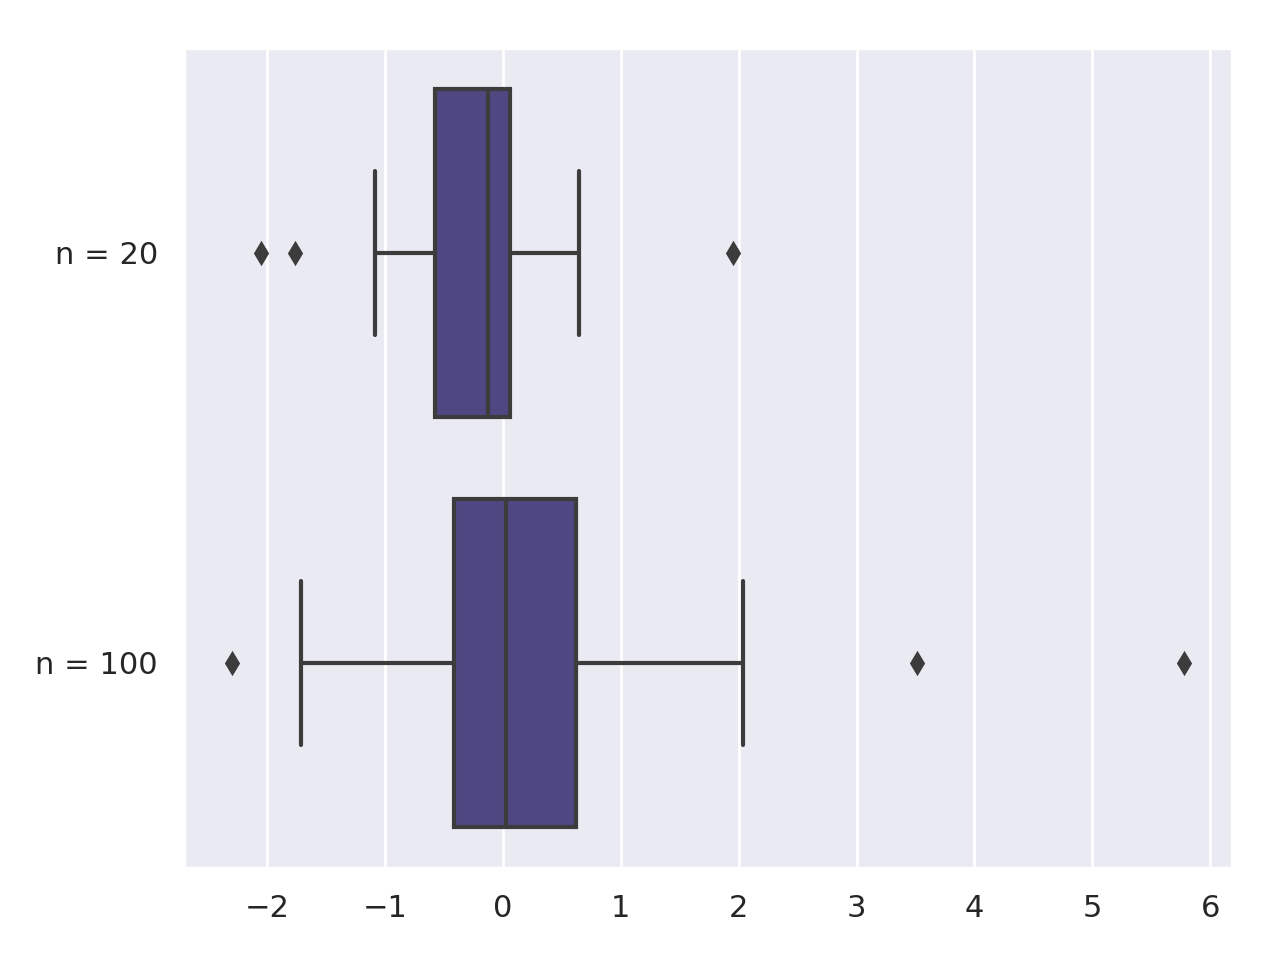
\includegraphics[width=13.cm, height=10.cm]{laplace}}
\label{pic:4}
\caption{Боксплот Тьюки для выборок из распределения Лапласа}
\end{figure}
\vspace{5.cm}

\textbf{Распределение Пуассона} с параметром $\lambda = 7$ 
\\
\begin{center}
    \begin{tabular}{ c | c | c }
        $$ & Практическая доля выбросов & Теоретическая доля выбросов  \\ \hline
        $n = 20$ & 0.0278 & 0.0027 \\ \hline
        $n = 100$ & 0.0119 & 0.0024 \\ 
    \end{tabular}
\end{center}

\begin{figure}[h!]
\centering
\center{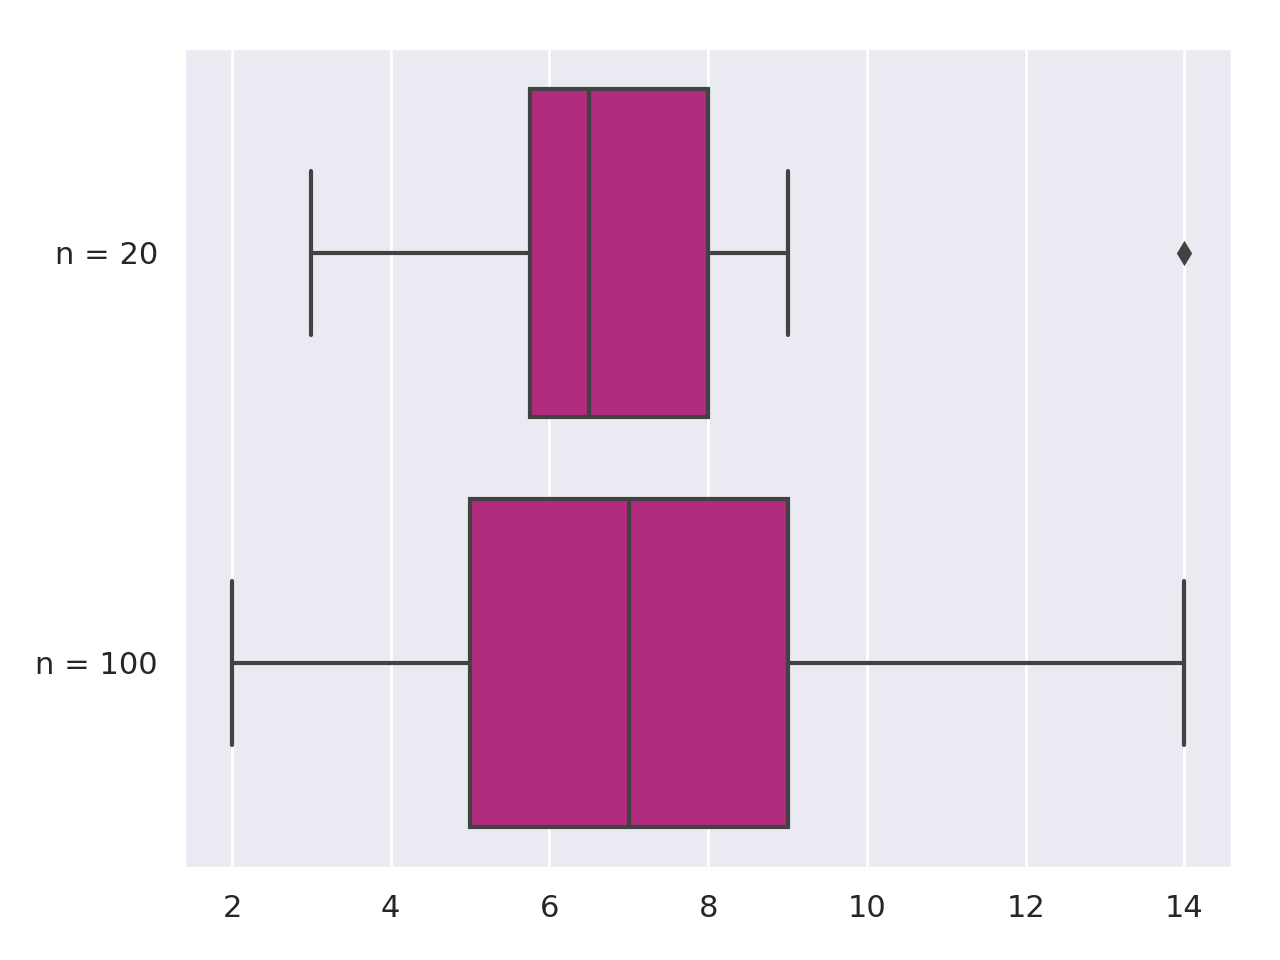
\includegraphics[width=13.cm, height=10.cm]{poiss}}
\label{pic:5}
\caption{Боксплот Тьюки для выборок из распределения Пуассона}
\end{figure}
\vspace{1.cm}

\indent{Взглянув на полученные результаты, можно сделать вывод о том, что равномерное распределение не имеет выбросов. Ненулевое значение в малой выборке при расчете квантилей с использованием значений выборки есть показатель того, что нельзя судить о характере распределения по выборке размером $n = 20$ окончательно. Отсутствие выбросов объясняется тем, что функция плотности такого респределения постоянна, и элемент выборки никогда будет вне отрезка, ограниченного \eqref{q:1}, \eqref{q:2}}

\indent{Наибольший процент выбросов установлен для выборов из распределения Коши. Также увеличение выборки не влияет на изменение результата, математического ожидания нет. Обратимся к результатам предыдущей лабораторной работы. Дисперсия размаха распределения на выборке $n = 100$ уже принимает значения порядка $10^8$. Это объясняет тот факт, что доля выбросов достаточно высока. Распределение Коши имеет тяжелые хвосты, и доля элементов, принимающих далекие от центра распределения значения, на порядок выше по сравнению с остальными распределениями, такими как нормальное, Лапласа, Пуассона.}


%%%%%%%%%%%%%%%%%%%%%%%%%%%%%%%%%%%%%%%%%%

\newpage
\begin{thebibliography}{}
    \bibitem{ms_1}\textit{Chrisman, L.} How the strange Cauchy distribution proved useful. \textit{Lumina Decision Systems} (2018). URL: http://www.lumina.com/blog/how-the-strange-cauchy-distribution-proved-useful
\end{thebibliography}


\end{document}{}